A common process that requires speed and precision is taking a collection of products, boxes, letters or parts, and breaking it into a set of collections that are related in some way. The sorting conveyor described in this text will take a collection of elements and break it into three other collections based on their sizes. Such a system has many areas of application but, to name one, consider a factory that produces a variety of products of different sizes. At some point the total production will need to be sorted and the conveyor sorting system ("System") is an option to accomplish that.

The System is recommended because it handles high production volumes, but also small ones, faster and in less space than having a team of employees would. The System also has very high accuracy and potentially costs less than maintaining a team to do the same job. In addition, the system is potentially safer to employees and machines than having materials handled manually. Overall, the System will give companies higher revenue.

The System is built to be incorporated to pre-existing production lines but it is also able to operate by itself. It can be installed and operated in common work areas as it will not incur any significant risk to personnel. However, it can be used in fully automated areas as it does not require any human interaction. See the following image.

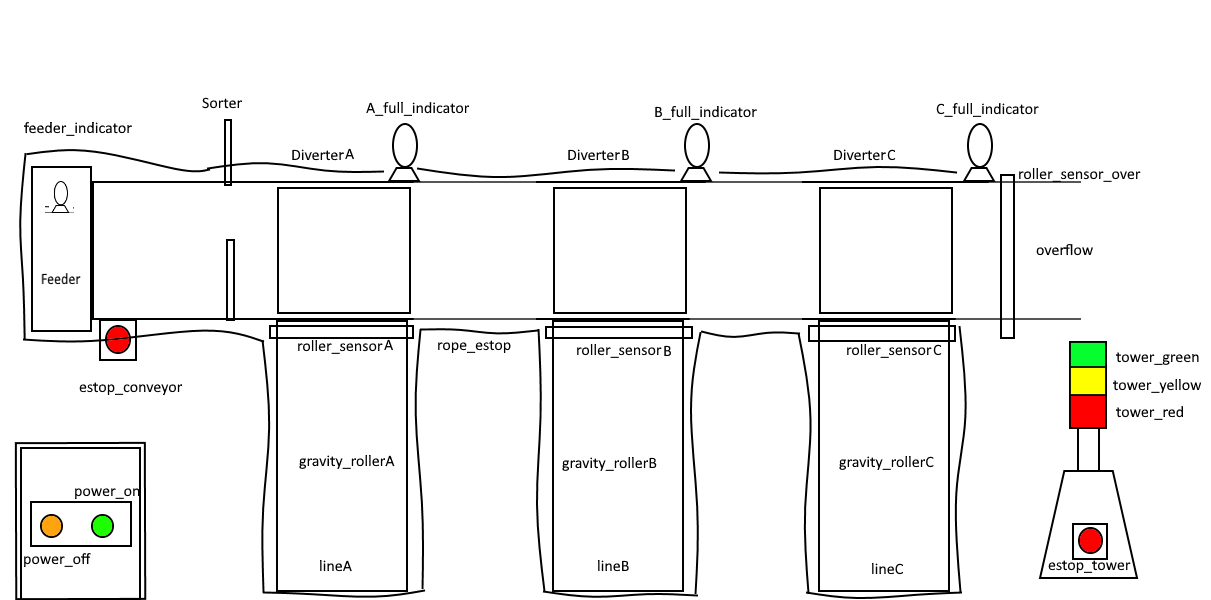
\includegraphics[scale=0.5]{../external/system_graphics_full.png}

Products will flow from the feeder, down to the belt and be sorted and moved, if possible, to their respective lines. If it is not possible to move to the designated area, the conveyor will transport the product to an overflow area. When shutting down or recovering from an emergency stop or power loss, the system will empty the conveyor by moving its products to the same overflow area.

When the feeder is filled with 12 products it will light an indicator light that lets the operator know the system can start running. If the feeder is not full, the system will not run. However, in order to successfully to startup, all emergency stops must also be reset in case they were activated. The first action taken when booting the system red lights will power on and horns will ring. 

After a delay, the system verifies, through internal PLC retentive counters, if it can power the main conveyor or if it should run a recover module. This decision is solely based on the count of products in the conveyor. If there are counter they will be moved to an overflow area. After startup the feeder will feed products at a constant rate until it goes empty. There are indicator lights for when the feeder becomes empty.

The products fed to the conveyor pass by an object detection and sizing sensor that will decide to which line is should go though. After that decision is made the PLC will coordinate the position of the belt diverters so that the products reaches the correct destination. The size is not the only factor in that decision, because if a line is full the PLC program will not allow the product to be moved there and will sent it to the overflow area instead.

A line is considered full either if its collection point capacity is reached or if some predefined total value of products is reached. Those predetermined values for the featured system are 36 for line A, 24 for line B and 18 for line C. The collection point capacity is also set to 8 and 6 for lines A and C, respectively, and unbounded for line B. When wither collection point is full, an indicator light will turn on the tower lights.

The internal counter that is used to decide if the main system can startup when the star push button is pressed works via sensors placed between the rollers of the lines and the overflow area. The count of products in the conveyor is the difference between the amount of projects that were moved from the feeder into the conveyor and the sum of the products that went through either of the four possible destinations.


Finally, when shutting down, normally, the system will make the same conveyor count verification and move of products done in the recovery module. That guarantees it can start safely in the next system startup but also makes sure no products is left behind inside the system, possibly unreachable. 

The final part of the system is the way it handles emergency stop. The current state of the implemented simulation will stop both the main routine and the recovery module immediately. While that is good, it could also trigger breaks on the conveyor instead of letting the inertia take effect. That is one point of improvement that will be discussed by the end of the proposal.










